\chapter{Neue Technologien und Regulatorik im Finanzwesen}
\label{ch:background}
Software hat eine Schlüsselrolle für digitale Innovation in allen Bereichen \cite{Alt2017}, die wichtiger denn je geworden ist. Die IT ist ständigen Veränderungen ausgesetzt. Technologietrends erzeugen immer wieder neue Impulse und Betriebe mit properietären Infrastrukturen müssen sich neu ausrichten \cite{Bussmann2006}.

So entstehen gegenüber etablierten Unternehmen, Technologieunternehmen mit effizienten Geschäftsmodellen. Sie integrieren mit unterstützenden Anwendungen IT und Geschäftsmodell \cite{Bussmann2006}. Im Finanzwesen sind es die sogenannten FinTechs \ref{Disruption:FinTechs}

Der nachfolgende Kapitel untersucht mithilfe einer Fallstudie innovative Technologien aus verschiedenen Perspektiven. Die Auswirkungen von neuen Technologien werden nach der Fallstudie weiter ausgeführt und ihre Eigenschaften hervorgehoben. Durch die zusätzliche Perspektive der Regulatorik auf neue Technologien werden Einschränkende und antreibende Faktoren für Innovation, insbesondere im Rahmen der \ac{SEU} im Finanzwesen werden identifiziert.

Mithilfe diesem werden Bereiche hervorgehoben, in denen ein Paradigmenwechsel erfolgen muss, um die Rahmenbedingungen innovationsfördernd zu verändern.

\section{Fallstudie Goldman Sachs}
\label{section:Goldman}
Goldman Sachs sieht sich nicht als Finanzdienstleister, sondern als ein Technologieunternehmen und als eine Plattform \cite{Gupta:2017}. Diese Transformation kann als Vorbild für Institute des deutschen Finanzwesens gesehen werden. Auf der einen Seite stehen die FinTechts, die sich Marktanteile im Privatkundenbereich sichern und zunehmenden Druck auf die etablierten Institute ausüben. Auf der anderen Seite richten sich anpassungsfähige Institute neu aus und etablieren sich mit Technologien und Plattformen in neue Geschäftsmodelle. 

Gupta und Simonds \cite{Gupta:2017} haben die Transformation von Goldman Sachs hin zu einem Technologieunternehmen beschrieben. Nachfolgend werden die wesentlichen Punkte aus dieser Studie untersucht.
%
\paragraph{Technologien und ihre Auswirkung im Finanzwesen}
Folgende Auswirkungen ergaben sich durch neue Technologien für Goldman Sachs und waren ein Impuls für Veränderung \cite{Gupta:2017}:
\begin{itemize}
    \item Daten und Metriken wurden wertvoller als die Instinkte der Händler.
    \item Die Auswirkung von Technologie im Finanzwesen verstärkte sich seit der Finanzkrise 2008 umso stärker
    \item Cloud, Open-Source Software und Schnittstellen führten zu einer erheblichen Reduzierung von Zeit und Kosten in der eigenen Entwicklung von Technologien
    \item Verstärkter Wettbewerb durch FinTechs
\end{itemize}

Ein interessanter Punkt ist vor allem die Reduktion der Kosten für die eigene Entwicklung von Technologien. Verwendung von Standardsoftware, die Open-Source ist, bringt die Softwareentwicklung auf einen gemeinsamen Nenner. Mit der Verwendung von Standardsoftware für die Entwicklung von Anwendungen können öffentliche Ansätze für einen spezifischen Bedarf angepasst werden. Probleme bezüglich der Skalierung von Anwendungen im Betrieb sind beispielsweise kein neues Problem. Zu gängigen Anwendungen wie Jenkins existieren öffentliche Ansätze \ref{fig:gkejenkins}, die auf den jeweiligen Bedarf angepasst werden müssen. Das Erspart sehr viel Aufwand in der Entwicklung eines eigenen Konzepts für den individuellen Bedarf. Die Verwendung von Standardsoftware, reduziert auch die Einstiegshürden der Fachkräfte. Properitäre Anwendungen benötigen dagegen spezialisiertes Personal. Open-Source und Standardsoftware sind somit ein Antreiber für die Softwareentwicklung.

Parallel dazu sind Cloud-Plattformen ein weiterer Antreiber für die Entwicklung von eigenen Anwendungen. Sie bieten eine Plattform für IT-Ressourcen, sodass eine Infrastruktur mit sofortiger Wirkung umgesetzt werden kann. Es gibt eine ganze Reihe an Begriffen für die Konzepte, die Cloud-Plattformen ermöglichen. Diese beinhalten \ac{IaaS}, \ac{IaC}, \ac{SaaS} und \ac{PaaS}.
Die Cloud-Technologie ist nicht nur eine standardisierende Möglichkeit für die seit langem angeforderte \ac{SOA} \cite{Brockhoff2006} in Banken. Sie ist möglicherweise Brandbeschleuniger für die digitale Transformation ganzer Branchen. Für Goldman Sachs war sie definitiv ein Treiber für die Entwicklung von offenen und flexiblen Plattformen.
%
\paragraph{IT-Strategie von Goldman Sachs}
Die Integration von neuen Technologien war für Goldman Sachs Opportunität und unvermeidbar \cite{Gupta:2017} zugleich:
\begin{itemize}
    \item Kostensenkung durch eine Effizienzsteigerung des Betriebs
    \item Entwicklung von internen und externen Plattformen
    \item Unterstützung des Kerngeschäfts
    \item Wertschöpfung von neuen Geschäftsmodellen
\end{itemize}

Gerade der verstärkte Wettbewerb durch FinTechs und der finanzielle Druck nach der Finanzkrise bedingten, dass sich das Unternehmen verändert. Die Unvermeidbarkeit dieser Entscheidung zeigt auch, dass Opportunitäten nicht ausreichen, um Veränderungen umzusetzen. Goldman Sachs musste sich anpassen, um in einer digitalen Welt geschäftsfähig zu bleiben. Sie musste neue Technologien integrieren, weil das alte Modell nicht mehr tragbar war. 

Der Ansatz neue Technologien anzunehmen hat weitreichende Auswirkungen für die Zukunft von Goldman Sachs \cite{Gupta:2017}. Eine gewisse Risikoakzeptanz von oft unvorhersehbaren Auswirkungen sollte vorhanden sein, um sich für neue Technologien zu überwinden. Handlungsunfähigkeit ist oft das größere Risiko. 

\paragraph{Effizienzsteigerung}
Wie \citet{Gupta:2017} erkennt, hat Goldman Sachs die Automatisierung von Geschäftsprozessen durch die Zentralisierung von Kernelementen vorangetrieben, wodurch Redundanzen entfernt wurden. 

Ezra Nahum\footnote{\citet{Gupta:2017} zitiert Ezra Nahum, S.5} betont, dass die unterschiedlichen Geschäfte von Goldman Sachs bisher in \enquote{Silos} als unabhängige und eigenverantwortliche Einheiten ausgeführt wurden. Es stellte sich die Frage, was ihre gemeinsamen Nenner sind. Ein Ansatz war in einer gemeinsamen technologischen Plattform zu arbeiten und in kleineren Teams sich darauf zu konzentrieren, was das jeweilige Geschäft ausmacht. Zu ihrer Unterstützung unterliegt ihnen ein größeres gemeinsamen Team \cite{Gupta:2017}.
\bigskip
\\
Verallgemeinert kann dieser Ansatz auch für die Effizienzsteigerung in anderen Bereichen genutzt werden. Zuerst werden gemeinsame Nenner identifiziert. Als nächstes werden sie ausgelagert. Das ermöglicht die Einrichtung einer gemeinsamen Plattformen, sodass sich Einheiten oder Komponenten auf ihre eigentliche Kernaufgabe konzentrieren. Es wird hierbei nach der konstruktiven Frage \enquote{Welche Gemeinsamkeiten haben wir?} statt nach der Frage \enquote{Was unterscheidet uns?} aufgebaut. Ersteres impliziert schon die Identifizierung von Gemeinsamkeiten, wodurch Redundanzen nicht unentdeckt bleiben und Synergie erzeugt wird. Die zweite Frage impliziert eine Abgrenzung der Einheiten voneinander, wodurch die \enquote{Silos} immer höher werden. Unterschiedliche Bedürfnisse müssen nicht zu unterschiedlichen Technologien führen. 

Bezogen auf die Anwendungsentwicklung können diese \enquote{Silos} auch als Metapher für die monolithischen Systeme \cite{Bussmann2006} aus dem Finanzwesen gesehen werden. Eine \ac{SOA} alleine reicht nicht aus, um mit kontinuierlichen Veränderungen der IT umzugehen. Die Anwendungen selbst müssen in kleinere funktionale Komponenten aufgeteilt werden \cite{Bussmann2006}. Microservice Architekturen bieten hierfür einen möglichen Ansatz. Die wesentlichen Funktionen für die Kernaufgabe einer Anwendung machen nur einen kleinen Teil der ganzen Anwendung aus. Unterstützende Tätigkeiten können unter gemeinsamen Plattformen zusammengefasst werden, wodurch auch neue Möglichkeiten entstehen. Ein Beispiel wäre eine gemeinsame Datenbank. Goldman Sachs konnte durch einen gemeinsamen \enquote{Data Lake} \ref{goldman:plattform} und Mashine-Learning die Marktdaten effektiver bewerten.
\medskip
\\
\citet{Gupta:2017} beschreibt, dass die Umsetzung dieser Strategie sich als schwierig gestaltet. Sie erfordert die Zusammenarbeit aller Beteiligten. Die verschiedenen Abteilungen müssen für die Umsetzung dieser Strategie kurzfristige Kompromisse eingehen und als finanziell eigenverantwortliche Einheiten die Kosten vorerst tragen. 

Cohen\footnote{\citet{Gupta:2017} zitiert Darren Cohen, S.5, aus dem Englischen übersetzt} betont hierzu das wesentliche Problem:
\begin{quote}\label{quote:goldman-vision}
    Die Vision ist eine Sache, aber der wirkliche Fortschritt besteht darin, die Organisation dazu zu bringen, die Barrieren abzubauen, um in einer digitalen Welt zu agieren und die traditionell tiefen vertikalen Barrieren zu überwinden
\end{quote}
\medskip
Ähnliche Probleme gibt es auch innerhalb der IT, insbesondere in der Zusammenarbeit zwischen Entwicklung und Betrieb \citet{Disterer2013}. Ansätze aus DevOps \cite{Alt2017} können hierbei die Zusammenarbeit innerhalb der IT verstärken. Im Finanzwesen wird für unvereinbare Verantwortungsbereiche eine strenge Funktionstrennng gefordert \cite{MaRisk:2017}.
Dies wirkt sich auch auf eine strikte Trennung zwischen Test- und Produktivumgebung aus \citet{MaRisk:2017} und könnte die Zusammenarbeit erschweren. Die Umsetzung der Funktionstrennung auch auf personeller Ebene für die IT begünstigt möglicherweise die Vertiefung von Barrieren und erschwert die Umsetzung von DevOps. Möglicherweise ist dies ein einschränkender Faktor für die Softwareentwicklung.

\paragraph{Technologieplattformen}
Goldman Sachs sah eine Opportunität darin, die internen Plattformen auch für ihre Kunden zugänglich zu machen. Darunter zählt die Plattform Marquee, die für interne Zwecke der Marktanalyse entwickelt wurde \cite{Gupta:2017}.
Die Anwendungen darin wurden self-contained entwickelt, sodass die Integration in interne und externe Systeme mit geringem Aufwand realisierbar war \cite{Gupta:2017}. Dadurch konnten die internen Plattformen schnell angepasst werden für neue Geschäftsmodelle. Die in der Plattform enthaltenen Anwendungen für die Marktanalyse konnten dadurch Geschäftskunden zugänglich gemacht werden, um den Kundendialog zu verbessern und Goldman Sachs zum bevorzugten Partner für Handel zu machen \cite{Gupta:2017}.
\medskip
\\
Was als interne Plattform angefangen hat konnte schnell umfunktioniert werden. Dies war durch ein offenes Design und geringen Abhängigkeiten der Plattform von Goldman Sachs möglich. Sie ist dabei den Kompromiss eingegangen eine wertvolle Anwendung unentgeldlich verfügbar zu machen, was kontrovers war. Im Gegenzug dafür war Goldman Sachs auf den lokalen Rechnern der Händler ihrer Geschäftskunden allgegenwärtig \cite{Gupta:2017}.

%
\paragraph{Technologien und Plattformen von Goldman Sachs}
\label{goldman:plattform}
\begin{itemize}
    \item \enquote{Data Lake} für Mashine-Learning durch eine \emph{hybride Cloud}\footnote{Gemeinsamer Einsatz einer extern und einer intern betriebenen Cloud-Plattform}
    \item \enquote{Marquee}, eine Bewertungsplattform für Marktanalysen
    \item \enquote{SIMON}, eine Plattform und Onlinemarktplatz für \enquote{Structured Notes}
\end{itemize}

\paragraph{neue Geschäftsmodelle}
Mit der Entwicklung von SIMON, einem Onlinemarktplatz für \enquote{Structured Notes}, erhöhte Goldman Sachs ihre Reichweite zu einer neuen Nutzergruppe. Das Wachstumspotenzial von einer Plattform mit einem einzigen Anbieter wurde erreicht, sodass die eigene Plattform an weitere konkurrierenden Emittenten geöffnet wurde. Dies erhöhte die Kundenzufriedenheit, da eine größere Auswahl und Vielfalt an Angeboten hierdurch entstand \cite{Gupta:2017}.

\paragraph{Ausblick}
\citet{Gupta:2017} fasst zusammen, dass die Realität nach 2008 Goldman Sachs und ihre Konkurrenz gezwungen hat sich neu auszurichten und wirft einige Fragen auf: \footnote{\citet{Gupta:2017}, S. 10, aus dem Englischen übersetzt}
\begin{quote}
\enquote{Einblicke in die Strategie von Goldman Sachs wurden durch Initiativen wie Marquee und Marcus deutlich, aber wie passten diese und andere Initiativen der letzten Zeit in das allgemeine Geschäftsmodell des Unternehmens? Hat sich das Kerngeschäft von Goldman Sachs verändert, oder waren Produkte wie SIMON und Marcus an der Peripherie angesiedelt? Was trieb das Unternehmen dazu, den Zugang zu internen Tools zu öffnen, die lange Zeit als proprietärer Wettbewerbsvorteil angesehen worden waren, und wie konnte es rechtfertigen, Wettbewerber zum Verkauf an seine Kunden einzuladen?
    }
\end{quote}
Die Realität nach 2008 könnte diese Fragen von sich aus beantworten. Hierzu sollten die veränderten Rahmenbedingungen der IT im Finanzwesen verstanden werden. Zudem ist die Realität zu erkennen, dass neue Technologien immer schneller entstehen und ihre Auswirkungen immer stärker werden. 
\medskip
\\
\citet{Eismann2015} beschreibt, dass aus den Plattformansätzen von Apple und Google einiges gelernt werden kann. Beide Unternehmen bieten Plattformen für Apps an und verdienen an ihrem Vertrieb deutlich mit. Dabei müssen sie die Apps nicht selbst entwickeln. Durch Plattformen findet eine \emph{Auslagerung von Innovation \cite{Eismann2015}} statt.

Daher ergibt es Sinn, dass Goldman Sachs sich die Plattformansätze von führenden Technologieunternehmen aneignet und selbst ein Ökosystem mit Plattformen aufbauen will. 

Vielen Banken scheint diese Idee jedoch fremd \cite{Eismann2015}.
\citet{Eismann2015} begründet, dass Kernbankensysteme niemals dafür ausgelegt wurden externe Software zu integrieren, was aus Sicherheitsgründen vertretbar ist, jedoch eine starke Limitation für Innovation aufgrund kostspieligen Anpassungen darstellt.
\medskip
\\
Alt et al. \cite{Alt2017} definieren, dass der aktuelle Innovationsverlauf auf \emph{Diskontinuitäten} beruht und disruptiv stattfindet und haben hierzu einen entscheidenden Vorschlag: \footnote{\citet{Alt2017}, S. 14}
\begin{quote}
\enquote{Für die Vorwegnahme künftiger Innovationen ist die Gestaltung künftiger
Zukunftszustände bzw. Verwendungszusammenhänge durch die zeitnahe Realisierung von Prototypen von besonderer Bedeutung.}
\end{quote}
Besonders sollte hierbei die Gestaltung \emph{künftiger Zukunftszustände \cite{Alt2017}} hervorgehoben werden. Das IT-Management muss in der Lage sein Technologietrends zu verstehen und ihre Auswirkungen auf ihr Geschäft zu transferieren. Dabei gibt es Unterschiede zwischen Diskontinuität und Disruption von Technologien \cite{Fernandez:2020}.  Die \emph{künftigen Verwendungszusammenhänge} sind hierbei für die Wertschöpfung von neuen Opportunitäten wichtig. Opportunitäten können jedoch verpasst werden, wenn sie nur eine Erweiterung von Geschäftsmodellen darstellen. Um die Kontinuität des Kerngeschäfts aufrecht zu erhalten sind die \emph{künftigen Zukunftszustände \cite{Alt2017}} essenziell. Für die zeitnahe Realisierung von Prototypen erfordert es kreative \cite{Alt2017} und schnelle Ansätze, wie zum Beispiel der \emph{Design Thinking} Prozess.

\section{Diskontinuität und Disruption}
Die unflexible IT-Architektur in Banken ist keine neue Erkenntnis und wird seit langer Zeit gefordert \cite{Brockhoff2006}, \cite{Bussmann2006}. Mittlerweile sollte herbei nicht mehr von Bedarf oder Forderung gesprochen werden. Die Opportunität für eine flexible \ac{SOA} ist bereits durch Cloud-Plattformen vergangen. Die geforderte \ac{SOA} wurde zuletzt durch Mircroservice-Architekturen ersetzt. Diese Beobachtung ist Beispiel für eine \emph{Diskontinuität} durch die Cloud-Computing Technologie.
\medskip
\\
Veränderungen werden nicht nur durch ein Wertschöpfungspotenzial hervorgerufen. Viel mehr wird die IT in Betrieben mit alten Strukturen durch äußere Kräfte gezwungen sich anzupassen \cite{Alt2017}, \cite{Gupta:2017}. Grundlage hierfür sind neue Technologietrends \cite{Bussmann2006}, die mittlerweile in ihrer Auswirkung jedoch gravierender sind. Eine entsprechende Verdrängung im Wettbewerb kann viel schneller erfolgen als bisher. Neben Impulse für Innovation mit gefolgter Diskontinuität \cite{Alt2017} kann zunehmend eine Disruption durch neue Technologietrends beobachtet werden. Fernández et al. \cite{Fernandez:2020} definieren die voneinander schwierig zu unterscheidenden Konzepte der \enquote{diskontinuierlichen} und \enquote{disruptiven} Technologien.
\medskip
\\
Verdrängungen im Wettbewerb finden nicht mehr durch eine Konkurrenz auf gleicher Augenhöhe statt. Eine Verdrängung kann auch unerwartet von kleinen Betrieben mit effizienten Abläufen kommen, die durch Schnelligkeit, Verfügbarkeit, Skalierbarkeit und Qualität ihrer Leistungen überzeugen kann.  Gerade im Bankwesen könnten Verdrängungen stattfinden, die jenseits der bisherigen Rahmenbedingungen agieren. Der hierfürige Technologietrend könnte im Finanzwesen beispielsweise die Blockchain-Technologie sein. Analog zum genossenschaftlichen Prinzip der Selbsthilfe, Selbstverantwortung und Selbstverwaltung könnten unabhängige Organisationen entstehen, nach dem historischen Muster, aus denen die Genossenschaftsbanken entstanden sind.
\medskip
\\
Die Vorwegnahme künftiger Innovation durch die Gestaltung von Zukunftszuständen \cite{Alt2017} ist ein Ansatz, um insbesondere Diskontinuitäten entgegen zu wirken. 
Für Disruptivität kann hierzu ein zusätzlicher Fokus ergänzt werden. Während der Gestaltung von Zukunftszuständen könnten Risiken für das Kerngeschäft mit kreativen Ausblicken auf disruptive Technologien antizipiert werden. Eine realistische Bedrohung auf den künftigen Zustand des Unternehmens könnte den nötigen Katalysator für einen Paradigmenwechsel liefern.

Nach einem erfolgreichen Paradigmenwechsel, durch die Erkennung der Bedrohungslage sollten disruptive Technologien mit den aktuellen Rahmenbedingungen abgeglichen werden. Dadurch könnten die Einschränkungen für Innovation identifiziert werden und es könnte definiert werden in welchen Bereichen ein Paradigmenwechsel erforderlich ist.

\paragraph{FinTechs}
\label{Disruption:FinTechs}
Aus den FinTechs entstehen mittlerweile volllizensierte Banken mit direktem Vertrieb über das Internet, wie zum Beispiel N26. Dazu entstehen Banken, die Schnittstellen für Unternehmen anbieten und somit eine reine Plattform für Finanzdienstleistungen sind, beispielsweise die Solarisbank. Auch etablierte Banken haben veränderte Rahmenbedingungen und Impulse erkannt und passen sich dem aktuellen Stand der Technik an \cite{Gupta:2017}, \cite{Eismann2015}.
\medskip
\\
Darren Cohen\footnote{Vorsitzender von Goldman Sachs' PSI Group, vgl. \cite{Gupta:2017}} sieht im Bereich Wertpapierhandel von FinTechs keine Gefahr für Goldman Sachs \cite{Gupta:2017}.
Hierzu wird in \cite{Gupta:2017} aufgeführt, dass laut Cohen die Anforderungen für neue Marktteilnehmer schwierig sind und für junge FinTechs unüberwindlich. In \cite{Gupta:2017} ist nach Cohen die Abwicklung im Bereich Wertpapierhandel hochreguliert und erfordert eine hohe Bilanzsumme, hohe Infrastrukturinvestitionen und einen erheblichen, globalen Einfluss.

Cohens Begründung pauschalisiert jedoch die Rahmenbedingungen der FinTechs. Abwicklungen mit hohen Summen finden bereits über Plattformen von Blockchain FinTechs statt. Diese Unternehmen agieren jenseits der Rahmenbedingungen und Regulierungen von konventionellen Instituten \ref{Disruption:Blockchain}.

\paragraph{Blockchain}
\label{Disruption:Blockchain}
Im Gegenzug zu Cohens Anforderungen für neue Marktteilnehmer \ref{section:Goldman} gelten einige Blockchains als hochgesichert, enthalten hohe Bilanzsummen, besitzen einer der vermutlich leistungsstärksten Infrastrukturnetzwerke weltweit und sind dadurch global in jeder Hinsicht.

An der \ac{DLT} können sich unter anderem FinTechs beteiligen und die Eintrittsbedingungen mit Leichtigkeit überwinden. Zu den bekanntesten Handelsplattformen, die aus der Blockchain-Technologie entstanden sind zählen Kraken, Poloniex, Bitfinex, Shapeshift und Coinbase. Abwicklungen in diesen Handelsplätzen finden nach \citet{Foundation2019Deconstructing} unter anderem dezentral mithilfe von Smart-Contracts und Reserven statt.

Die \ac{DLT} wird auch von etablierten Instituten im Finanzwesen genau verfolgt.
Für die Abwicklung von Schuldscheindarlehen existiert jüngst das deutsche Pilotprojekt finledger \cite{finledger}. 
Basierend auf der \ac{DLT} erschafft ein Konsortium aus deutschen Kreditinstituten die Plattform finledger, die zu einem Standard werden und nach der Pilotierung allen Instituten zugänglich sein soll \cite{finledger}.

\begin{figure}[htbp]
 \centering
 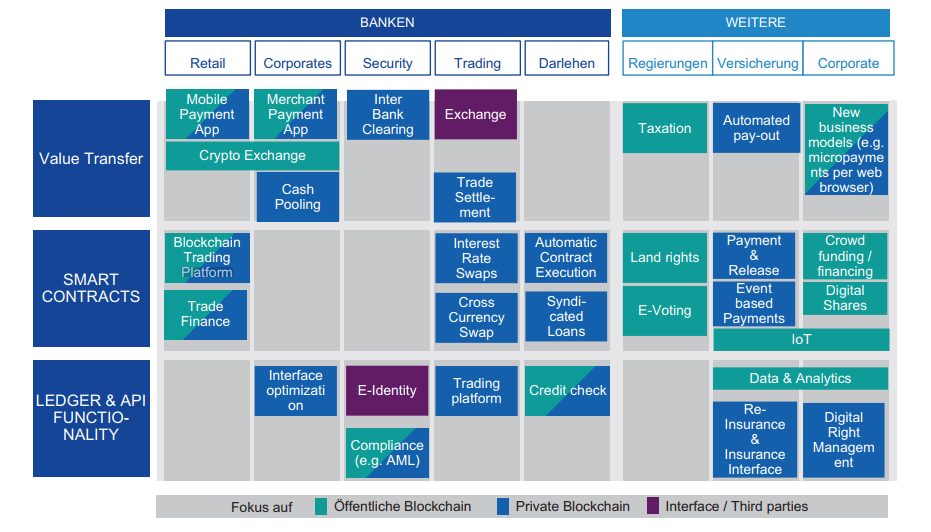
\includegraphics[width=1.0\textwidth]{gfx/blockchainanwendung.PNG}
 \caption{Korschinowski et al. \cite{Korschinowski2018}, S. 283, \enquote{Anwendungsfelder der Blockchain-Technologie. (Quelle: KPMG)}\label{fig:blockchain}}
\end{figure}

In Abb. \ref{fig:blockchain}, die Korschinowski et al. \cite{Korschinowski2018} übernommen haben wird ein Überblick der Anwendungsgebiete der \ac{DLT} gezeigt. In einigen Anwendungsbereichen hieraus könnten Ideen für zukünftige Plattformen nach der Vision von Goldman Sachs \ref{quote:goldman-vision} entstehen. Besonders in bankfachlichen Anwendungsgebieten müssen neue Technologien mit der Regulatorik abgewägt werden.

\paragraph{Software Development \enquote{as a Service}}
Eine künftige Disruption würde möglicherweise als Folge auf die Auslagerung und Dematerialisierung fast aller Komponenten in der IT entstehen.
Es stellt sich die Frage ob der Entwickler oder die Entwicklungsarbeit selbst als eine vollautomatisierte Dienstleistung bereitgestellt werden kann. Dieses zukünftige Konzept könnte als Trend \enquote{Software Development as Code} oder sogar \enquote{Software Development as a Service} genannt werden, als Folge auf die neuen Rahmenbedingungen durch Cloud-Architekturen. Gemeint ist hierbei eine mögliche Abstraktion und Vollautomatisierung der Entwicklungsarbeit.
Der Begriff \enquote{Software Development as a Service} existiert bereits im Rahmen einer Serviceorientierung der Entwicklung durch agile Methoden \cite{Lehman:2011}.

\emph{Freelancing} und \emph{Consulting} ist verbreitet in der IT und kann insbesondere aufgrund der zunehmenden Möglichkeiten und Akzeptanz für Remote-Arbeit sich immer weiter entwickeln. Möglicherweise könnte nach einer Transformation der gesamten IT-Architektur hin zu einer Cloud-Architektur eine Disruption oder Diskontinuität entstehen mit unvorsehbaren Auswirkungen auf die IT. Cloud-Plattformen bieten eine Architektur, die allgegenwärtig und fortschrittlicher sein wird. Entwicklungs- und Produktivumgebungen werden weiterhin streng getrennt sein müssen \cite{MaRisk:2017}. Das ist jedoch kein Hindernis für neue Geschäftsmodelle in der Softwareentwicklung, so lange eine kontinuierliche Zusammenarbeit zwischen diesen Bereichen besteht.

Zukünftig könnten Plattformen entstehen, die Entwicklungsarbeit abstrahieren und durch sichere Zugänge auf die Cloud-Architektur dem Kunden zur Verfügung stellen. Ihre Bedingung ist die Rückverfolgbarkeit von Ergebnisartefakten im Softwareentwicklungsprozss, mithilfe von Automatisierung und Nachvollziehbarkeit der Delivery Pipeline. Durch den Zugang einer Instanz der Entwicklungsumgebung gegenüber diesen Plattformen könnten Dienstleistungen für Entwicklungsarbeit analog zum Cloud-Computing gebucht werden.

Je nach Auslegung und Perspektive wäre diese beispielhafte Vorstellung eine Innovation oder Gefahr. Um ihr zu entgegnen sollte das Szenario durchgegangen werden. Für Entwickler entstehen möglicherweise Opportunitäten oder auch Risiken. 
\medskip
\\
Solche Entwicklungen werden unvermeidbar sein und zeigen sich zuerst in Form von Impulsen \cite{Bussmann2006} und nehmen mit zunehmender Reife der Technologie eine disruptive Eigenschaft an. Die genannten Beispiele für disruptive und diskontinuierlichen Technologien zeigen, dass die Entwicklung keinen Halt macht und ständig fortgeführt werden kann.

\section{Regulatorik der IT}
Die \emph{Finanzkrise 2008} war mit einem enormen Vertrauensverlust gegenüber Banken verbunden und die Empörung der Gesellschaft war durch das Internet und der daraus folgenden Transparenz viel größer als zuvor \cite{Eismann2015}. Eine Welle von regulatorischen Veränderungen wurde durch die Auswirkungen dieser Krise herbeigeführt, um zukünftige systemische Krisen zu vermeiden \cite{Gupta:2017}. Das Ergebnis daraus ist die Steigung der regulatorischen Anforderungen mit gleichzeitiger Zunahme der technischen Anforderungen\footnote{insbesondere der \enquote{kontinuierliche Anstieg der Anforderungen an die IT-Architektur} \cite{Disterer2013}} in der IT. 
Daraus resultiert ein zunehmender Druck auf das Finanzwesen (Abb. \ref{fig:bankdruck}), der aus zusätzlichen Kosten und wirtschaftlichem Druck besteht \cite{Smolinski2017}.

\paragraph{BaFin Anforderungen}
Aus dem \ac{KWG} der Bundesrepublik Deutschland entstehen Anforderungen an Kredit- und Finanzdienstleistungsinstitute, die sich auch auf die IT der Banken auswirken. Im \ac{KWG} wird die BaFin für die Aufsicht der Institute nominiert. Sie veröffentlicht Vorgaben an die von ihr beaufsichtigten Institute, um eine einheitliche Verwaltungspraxis sicherzustellen, mit der sich die Institute auf die Prüfungen der BaFin einstellen \cite{BaFin:Verwaltungspraxis}. 

Die BaFin präzisiert in \cite{MaRisk:2017} die Anforderungen des \ac{KWG} im Bereich Risikomanagement und Auslagerung. In \cite{BAIT:2018} werden diese Anforderungen für den Bereich der IT nochmals konkretisiert. Hierdurch sollen operationelle Risiken auch in der IT angemessen gesteuert werden. \citet{mci/Knittl2013} beschreibt die Umsetzung dieser Anforderungen anhand einer Fallstudie zu einem internationalen Finanzkonzern, worauf am Ende dieses Abschnitts eingegangen wird (\ref{section:regulatorik-umgang}).

\begin{figure}[htbp]
 \centering
 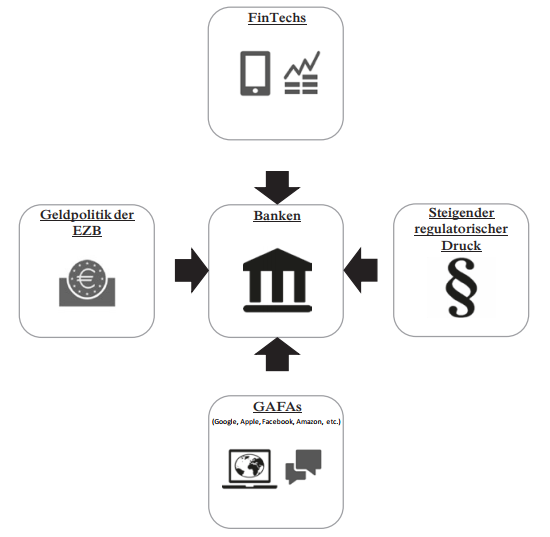
\includegraphics[width=0.8\textwidth]{gfx/bankdruck.PNG}
 \caption{\citet{Smolinski2017}, S. 44, Finanzbranche unter Druck}\label{fig:bankdruck}
\end{figure}

\medskip
Abb. \ref{fig:bankdruck} verbildlicht, wie Banken von allen Seiten unter Druck stehen. Die Darstellung könnte fortgeführt werden mit der Annahme, dass die äußeren Kräfte sich auch gegenseitig befeuern. Die Technologien und Trends aus den \enquote{GAFAs} können mit Sicherheit als ein Antreiber für die FinTechs gesehen werden. Die Antreibendenden Faktoren auf der vertikalen Achse der Abbildung werden von einschränkenden Faktoren auf der horizontalen Achse durchkreuzt. Die Aufsichten evaluieren ebenfalls neue Technologien und berücksichtigen sie jeweils bei der Novellierung ihrer Rahmenwerke. Bis diese angepasst werden vergeht Zeit und bis sich die etablierten Institute hierauf auch anpassen vergeht ebenfalls wertvolle Zeit. In FinTechs ist dieses Problem aufgrund ihrer Agilität und Effizienz geringer. Etablierte Institute müssen daher einen Weg finden das Zusammenspiel zwischen neuen Technologien und regulatorischen Anforderungen zu antizipieren und eigene Initiativen als Pilotprojekte schon zu starten. Hierzu passt ebenfalls der Ansatz der Vorwegnahme durch die Gestaltung von Zukunftszuständen \cite{Alt2017}.


\paragraph{Ermessen der Institute}
In \cite{MaRisk:2017, BAIT:2018} fällt auf, dass viele Vorgaben durch entsprechende Wörter in ihrem Gewicht relativiert werden. Die Maßnahmen zu ihrer Umsetzung liegen hierbei im Ermessen der jeweiligen Institute. Im Interesse der Institute ist in erster Linie das Bestehen von Prüfungen der Aufsicht. Die Ermessensfreiheit könnte in einigen Bereichen für Unklarheit sorgen, da die \ac{MaRisk} sehr abstrakt formuliert ist.
Eine bürokratisierte Kultur innerhalb der internen Kontrollverfahren in Kredit- und Finanzdienstleistungsinstituten zum bestehen von Prüfungen sollte als Folge vermieden werden. Die Flexibilität, die die BaFin in ihren Rahmenwerken vorsieht \cite{MaRisk:2017} sollte als stärke wahrgenommen werden und auf die interne Kultur übertragen werden. Die internen Kontrollverfahren und das Risikomanagement müssen in erster Linie praxisnah und flexibel bezüglich der IT vorgehen und ihren Ermessensspielraum zu Nutze machen, um mit neuen Technologien umgehen zu können.

Für die \ac{MaRisk} gibt es auch zusätzliche Erläuterungen der BaFin \cite{MaRiskErläuterungen:2017}. Speziell für die IT hat die BaFin in \cite{BAIT:2018} die \ac{MaRisk} noch einmal konkretisiert. Daneben gibt es institutspezifische Interpretationen und Werke, wie zum Beispiel vom Deutschen Sparkassen- und Giroverbund \cite{DSGV:2019}. Diese sollten jedoch als Best-Practice für eine begrenzte Zeit gesehen werden, da die Rahmenbedingungen sich ständig ändern.

\paragraph{Risikomanagement}
Für das Risikomanagement fordert die \ac{BaFin} die Festlegung von Strategien und die Einrichtung von internen Kontrollverfahren, bestehend aus einem \ac{IKS} und einer interne Revision. Ein Risikomanagement für die IT soll insbesondere den Betrieb schützen \cite{MaRisk:2017}, da hierin die operationellen Risiken liegen. Ein Ausfall der IT-Systeme in Banken hätte mit Sicherheit Auswirkungen auf kritische Geschäftsprozesse, die bis hin zu einer systemischen Krise führen könnten.

Daher fordert die \ac{BaFin} \cite{MaRisk:2017} vom IT-Risikomanagement:
\begin{enumerate}
    \item Sie soll Überwachungs- und Steuerungsprozesse für IT-Risiken einrichten.
    \item Ihre Prozesse umfassen: Risikokriterien, Risiken, Schutzbedarf, Schutzmaßnahmen, Risikobehandlung und -minderung
    \item Sie soll Risiken beim Einkauf von Software \emph{angemessen} bewerten.
\end{enumerate}
Diese Forderungen \cite{MaRisk:2017} zur Bewertung von IT-Risiken gelten auch beim Einsatz von selbst entwickelten Anwendungen, die von ihr als \ac{IDV} bezeichnet wird. Entsprechende Maßnahmen sollen jedoch nach dem Schutzbedarf der unterstützten Prozesse und verarbeiteten Daten festgelegt werden \cite{MaRisk:2017}.

Die Ermessensfreiheit zu den Maßnahmen des Risikomanagements begrenzt sich in diesem Fall auf den Schutzbedarf der Geschäftsprozesse und Daten. Die Überwachungs- und Steuerungsprozesse für IT-Risiken sollten daher klare Grenzen für die Verarbeitung von Daten definieren. Eine klare Unterscheidung zwischen \ac{IDV} Anwendungen und Anwendungen die keine \ac{IDV} darstellen ist nötig, um angemessene Maßnahmen festzulegen.

\paragraph{IT-Systeme und Prozesse}
Die \ac{BaFin} \cite{MaRisk:2017} fordert zu IT-Systemen und Prozessen:
\begin{enumerate}
    \item IT-Systeme und Prozesse sollen Integrität, Verfügbarkeit, Authentizität und Vertraulichkeit der Daten mit gängigen Standards sicherstellen.
    \item IT-Systeme und ihre zugehörigen Prozesse sollen hinsichtlich ihrer Eignung regelmäßig überprüft werden.
    \item IT-Systeme sollen nach \emph{wesentlichen} Veränderungen und vor erstmaligem Einsatz getestet werden.
    \item Ein Regelprozesse der Entwicklung, des Testens, der Freigabe und der Implementierung in die Produktionsprozesse soll etabliert werden. 
    \item Produktions- und Testumgebungen sollen grundsätzlich voneinander getrennt werden.
\end{enumerate}
%
Besonders hervorzuheben ist die Verantwortung der IT-Systeme und Prozesse für die Sicherstellung der Datensicherheit. Im Fokus stehen die verarbeiteten und gespeicherten Daten in den IT-Systemen und Prozessen. 

Hierzu fordert die BaFin \cite{MaRisk:2017} eine Orientierung am Schutzbedarf der verarbeiteten Daten. Sie verweist mit gängigen Standards auf den IT-Grundschutzkatalog\footnote{vgl. IT-Grundschutzkompendium \cite{IT-Grundschutz:2020}} des \ac{BSI} und auf den internationalen Sicherheitsstandard ISO/IEC 2700X\footnote{vgl. Disterer \cite{Disterer2013}} der \ac{ISO}.

Die Auslagerung von IT-Ressourcen wäre beispielsweise bei der Entwicklung von Modellen für Mashinelles-Lernen nötig und dürfte aufgrund der Datensicherheit nicht ohne weiteres auf einer externe Cloud-Plattform durchgeführt werden. 

Auch im Bereich der Automatisierung von Prozessen ist es wichtig zu erkennen, welche unterstützten Prozesse schutzbedürftig sind und welche nicht. Prozesse können zwischen \emph{Change} und \emph{Run} unterteilt werden. Die Run-Prozesse regeln den Betrieb und die Change-Prozesse erzeugen üblicherweise als Projekte Veränderungen im Aufbau oder Ablauf der Organisation.

Die Softwareentwicklung selbst enthält innerhalb einer getrennten Testumgebung auf dem ersten Blick keine operationellen Risiken für den Geschäftsbetrieb einer Bank und könnte als Change-Prozess klassifiziert werden können. Für die Implementierung von Ergebnissen aus diesen Change-Prozessen ist eine vorherige Freigabe vorgesehen, beispielsweise in Form von \enquote{Quality-Gates} \cite{mci/Disterer2011}.

Für ihre Unterstützung existiert jedoch innerhalb der IT ein umfangreicher Betrieb für Plattformen und Anwendungen der Softwareentwicklung. Ein hoher Schutzbedarf der Entwicklung entsteht in Prozessen für die Inbetriebnahme von Software. Besonders ist in der Anwendung von DevOps die Delivery-Pipeline, womit die Komponenten in die Produktionsumgebung integriert werden ein kritischer Prozess. Nach DevOps sind die Abläufe zwischen \ac{CI} und \ac{CD} für einen automatisierten und hochfrequenten Ablauf eng miteinander verbunden. Es stellt sich die Frage wie Anwendungen zur Ausführung der Delivery Pipeline einzuordnen sind. Für die Einhaltung der Funktionstrennung \cite{MaRisk:2017} zwischen Entwicklung und Betrieb müssen klare Grenzen gesetzt werden. 

\paragraph{Einschränkungen in der SEU}
Diese Grenzen sind nötig, um eine klare Nachvollziehbarkeit der Ergebnisse aus den Change-Prozessen zu bewahren. Besonders schwierig wird es im Rahmen der Regulatorik, wenn innerhalb der \ac{SEU} die Rollen schwierig voneinander zu unterscheiden sind. Konfiguration, Administration, Wartung und Weiterentwicklung von Anwendungen für den Betrieb der \ac{SEU} sind Tätigkeiten in denen Kunde, Entwickler und Betrieb (Abb. \ref{fig:devops}) teilweise miteinander verschmelzen. Auch die Überwachungsprozesse werden meist von den gleichen Entwicklern in der \ac{SEU} technisch umgesetzt. Die Auslagerung der \ac{SEU} auf externe Infrastrukturen gestaltet sich aufgrund dieser engen Kopplung sehr schwierig, weil hierdurch sensible Daten extern ausgetauscht werden und eine zu hohe Abhängigkeit für den Betrieb der Softwareentwicklung entsteht. Realistischer ist es nur einzelne Services auszulagern.
Monolithische Systeme sind für die \ac{SEU} keine skalierbare Lösung. Für automatisierte Prozesse und skalierbare, flexible Umgebungen können die Anwendungen aus der \ac{SEU} in noch kleinere Module aufgeteilt werden. Insbesondere ist es wichtig, dass einzelne Komponenten der Integrationsplattform trennbar sind und unabhängig voneinander laufen. Komponenten, die \enquote{self-contained} sind flexibler können auch unabhängig voneinander skaliert werden. Das würde Engpässe erheblich reduzieren. Die Eliminierung von Abhängigkeiten sorgt auch für eine bessere Nachvollziehbarkeit, da hierbei gängige Standards angewendet werden können.
Selbst wenn die Funktionstrennung mit neuen Technologien wie Container-Virtualisierung realisierbar ist, entstehen für die Verwendung von externen Cloud-Plattformen Probleme bezüglich der Datensicherheit. Die 

\paragraph{Wesentliche Veränderungen}
Die BaFin fordert, dass vor wesentlichen Veränderungen in der Aufbau- und Ablauforganisation sowie in den IT-Systemen das Institut die Auswirkung der geplanten Veränderung auf die Kontrollverfahren und -intensität zu analysieren hat. Hierfür sind die später in die Arbeitsabläufe eingebundenen Organisationseinheiten einzuschalten. Risikocontrolling, Compliance und die Interne Revision sind auch zu beteiligen \cite{MaRisk:2017}. 
%
\paragraph{Veränderung}
Daraus könnte ein Hindernis für solche Veränderungen entstehen. Wesentliche Veränderungen in den IT-Systemen könnten einen Anpassungsbedarf des Kontrollverfahrens bedeuten. Vielmehr sollte das interne Kontrollverfahren von einer ständigen Veränderung in der IT ausgehen.

\paragraph{Bankaufsichtliche Anforderungen an die IT}
Die \ac{BAIT} gibt seit 2018 neben der \ac{MaRisk} auf der gleichen Grundlage des \ac{KWG} einen  Rahmen, insbesondere für das Management der IT-Ressourcen und das IT-Risikomanagement. Die Anforderungen aus \ac{MaRisk} werden lediglich konkretisiert. Zudem Präzisiert es die Anforderungen des § 25b des
\ac{KWG} zu Auslagerung von Aktivitäten und Prozessen \cite{BAIT:2018}.
\\
Die \ac{BAIT} ist daher besonders für die Auslagerung von IT-Ressourcen zu berücksichtigen und insbesondere aufgrund der zunehmenden Praxis von \ac{SaaS} und Cloud-Computing relevant.
\\
Für die in dieser Arbeit durchgeführten Untersuchung zu einschränkenden Faktoren und Anforderungen daraus resultierender Anforderungen an die IT-Architektur werden einige Themen aus der \ac{BAIT} zusammengefasst.


\paragraph{IT-Strategie} Zunächst wird angefordert, dass die Geschäftsleitung eine nachhaltige IT-Strategie festlegen soll. Diese soll konsistent mit der Geschäftsstrategie sein \cite{BAIT:2018}. 
Aus den Mindestinhalten der geforderten IT-Strategie wird deutlich, dass Geschäftsmodell und IT in einem engen Verhältnis gesehen werden. Die IT steht aus regulatorischer Sicht nicht mehr größtenteils als Risikofaktor im Fokus. Vielmehr kann sie aufgrund einer konkreten Strategie das Geschäftsmodell ergänzen. Diese Anforderung ist eine klare 

\paragraph{IT-Governance} Die IT-Governance wird als Struktur zur Steuerung und Überwachung des IT-Betriebs und der Entwicklung der IT-Systeme und Prozesse auf Basis der IT-Strategie \cite{BAIT:2018} gesehen. Für das Risikomanagement, Entwicklung und Betrieb innerhalb der IT wird eine qualitativ und quantitativ angemessene Ausstattung mit Personal gefordert.

    

\paragraph{EBA Guidelines on ICT and security risk management}

\subsection{Umgang mit der Regulatorik}
\label{section:regulatorik-umgang}